

\subsection{Query Completion}
\label{sec:completion}

\enlargethispage{5pt}
\vspace{-1mm}

In this step, \ourtool completes the missing parts
in each query skeleton and outputs a list of SQL queries
that satisfy the given input-output examples.

% query conditions, the
%\CodeIn{GROUP BY} and \CodeIn{HAVING} clause (Section~\ref{sec:condition}),
%aggregates (Section~\ref{sec:agg_search}), and
%the \CodeIn{ORDER BY} clause (Section~\ref{sec:orderby})
%in each query skeleton, and
%outputs a list of SQL queries
%that satisfy the given example input and output pair.


%The SQL skeleton produced by the first step, though incomplete,
%serves as a good reference in inferring complete and valid SQL queries.
%In this step, our technique the remaining incomplete parts: conditions and
%aggregates, by rule-based learning and type-directed search, respectively.

\subsubsection{Inferring Query Conditions}
\label{sec:condition}

\ourtool casts the problem of \textit{inferring query conditions} as
 \textit{learning appropriate rules} that can perfectly divide a search space
into a positive part and a negative part. In our context, the search space
is all result tuples created by joining query tables; the positive part
includes all result tuples that contain the output table; and the negative part includes the remaining tuples.

The standard way for rule learning is using a decision-tree-based
algorithm. However, a key challenge is how
to design a sufficient set of features to capture relevant
relations between the example input and output.
Existing approaches~\cite{Tran:2009} simply use
tuple values in the input table(s) as features, 
and thus limit their abilities in inferring non-trivial
conditions. In particular,
merely using tuple values as features can only infer
conditions comparing a column value with a constant
(e.g., \CodeIn{student.level = 'senior'}), but
fails to infer conditions using aggregates (e.g., \CodeIn{COUNT(enrolled.course\_id) > 2}),
or conditions comparing values of two table columns
(e.g., \CodeIn{enrolled.course\_id > enrolled.score}).
This is primarily because tuple values from the input table(s)
do not include enough knowledge about the consequence of
applying an aggregate and the potential relations between
table columns.


To address this challenge, \ourtool 
adds two new types of features to each tuple,
and uses them together with the existing tuple values
for rule learning. The new features explicitly
encode useful information about SQL aggregates and
table column relations.

\begin{itemize}

\vspace{-1mm}

\item {\textbf{Aggregation Features}}. For each
column in the joined table, \ourtool 
groups all tuples by \textit{each} tuple's
value, and then applies every applicable aggregate\footnote{
\CodeIn{COUNT}, \CodeIn{COUNT DISTINCT}, \CodeIn{MAX},
\CodeIn{MIN}, \CodeIn{SUM}, and \CodeIn{AVG} for a
column of numeric type ;
and \CodeIn{COUNT}, and \CodeIn{COUNT DISTINCT} for
a column of string type } to each of the
 \textit{remaining} columns to compute the corresponding aggregation result. 
The ``Aggregation Features'' part in Figure~\ref{fig:features}
shows an example.

\item {\textbf{Comparison Features}}. For each tuple,
\ourtool compares
the values of every two type-compatible columns, and records
the comparison results ($1$ or $0$) as features.
The ``Comparison Features'' part in Figure~\ref{fig:features}
shows an example.

\end{itemize}

%The above two additional features seamlessly encodes SQL
%structure
% knowledge encoding permits our technique
%to make use of correlations between columns, rather than only values
%from each isolated and sequential columns.
%Table~\ref{tbl:com} shows an example.


%Using both tuple values and the enhanced features,
\ourtool employs a variant of the decision tree algorithm,
called PART~\cite{Frank:1998}, to learn a set of rules
as query conditions. We chose PART
because it uses a ``divide-and-conquer'' strategy to 
build rules incrementally, and thus is faster
and consumes less memory than
the original decision tree algorithm~\cite{Quinlan:1986}.
Using the new features added by \ourtool, the
PART algorithm is able to discover rules that are
hard to identify by only using the original tuple values as features.
Figure~\ref{fig:fullexample} shows an example.
%how such additional features
%help in learning rules for the motivating
%example in Figure~\ref{fig:motivating}.


%\todo{The incerasing number of features, can be falsified quickly,
%more features permits undiscover more rules}
%Figure~\ref{fig:fullexample} shows an example, in
%which the expected query condition uses the \CodeIn{COUNT} aggregate.


\begin{figure*}[t]
  \centering
  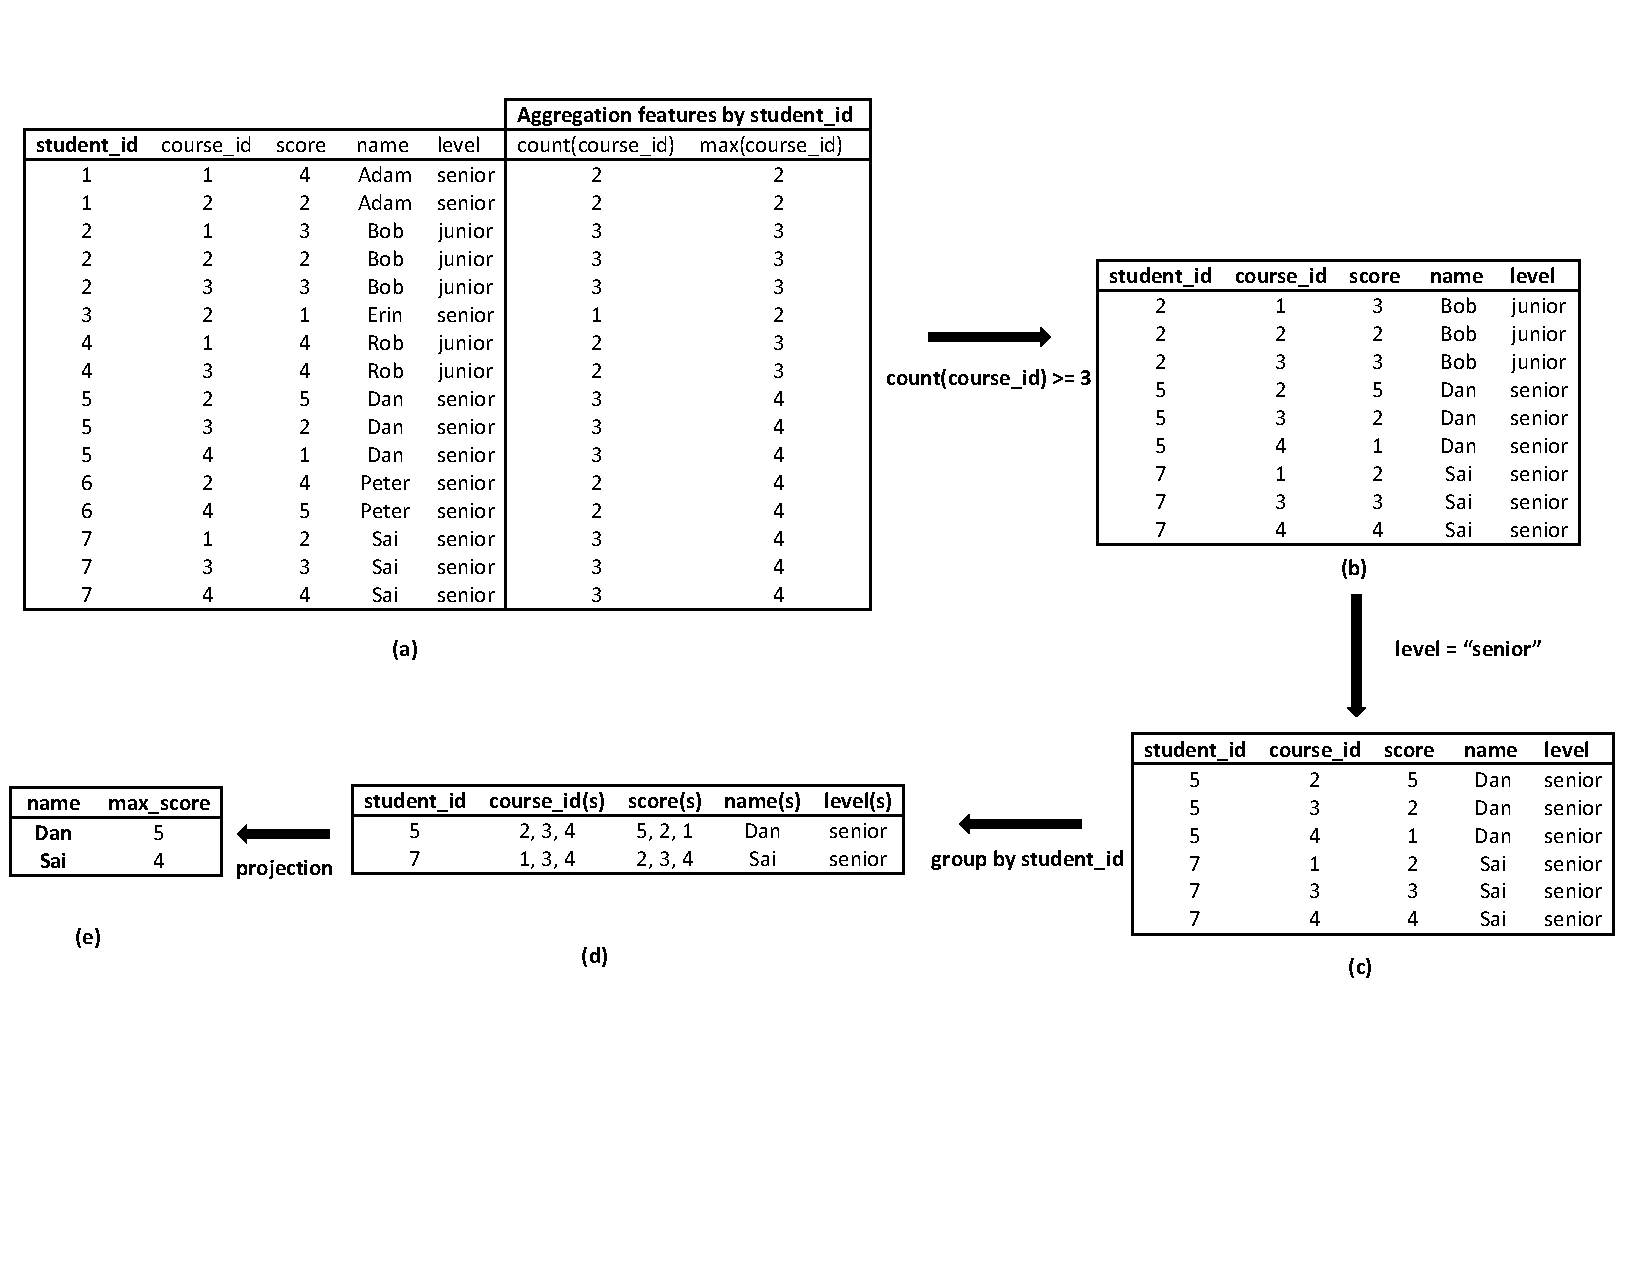
\includegraphics[scale=0.65]{fullexample}
  \vspace*{-2.0ex}\caption {{\label{fig:fullexample}
  Illustration of how the new features added by \ourtool
  help in inferring query conditions for the example in Figure~\ref{fig:motivating}.
  (a) shows \ourtool
  enriches the original tuple values (Left)
  with new features (Right). For brevity, only relevant
  aggregation features are shown. Using the added aggregation
  features, \ourtool observes that tuples whose feature values satisfy
  \CodeIn{COUNT(course\_id)>2} and \CodeIn{level=`senior'}
  appear in the output table,
  and thus infers a query condition that
  transforms the original table into the table shown in (b),
  which contains the output table shown in (c).
  Such query condition is difficult to discover 
  without using the aggregation features.
  (c) shows the output table, which is produced by projecting the
   table in (b) on the \CodeIn{name} column and the
  \CodeIn{MAX}(\CodeIn{score}) aggregate.}}
  \vspace{-1mm}
\end{figure*}


\ourtool splits the learned conditions into two disjoint parts,
and places each part to the appropriate clause.
Specifically, \ourtool places conditions
using aggregates to the \CodeIn{HAVING}
clause, and places other conditions to the \CodeIn{WHERE} clause.
This is based on the SQL language specification:
query conditions using aggregates are valid only when they
are used {together with} the \CodeIn{GROUP BY} clause
and are used in the \CodeIn{HAVING} clause.
Take the conditions inferred in Figure~\ref{fig:fullexample}
as an example, \ourtool puts the query
condition: \CodeIn{student.level =`senior'}
to the \CodeIn{WHERE} clause,
puts condition: \CodeIn{COUNT(enrolled.course\_id) > 2}
to the \CodeIn{HAVING} clause, and puts 
column \CodeIn{student\_id} to the \CodeIn{GROUP BY} clause.




%\end{itemize}

\subsubsection{Searching for Aggregates}
\label{sec:agg_search}

For every column in the output table that has no matched
column in the input table(s),
\ourtool searches for the desired aggregate by
repeatedly applying each aggregate on
every input table column; and checks whether
the aggregate produces the same output 
as in the output table. To speed up the exhaustive search,
\ourtool uses two sound heuristics to filter away infeasible
combinations.


\begin{itemize}
\item \ourtool only applies an aggregate
to its \textit{type-compatible} table columns. Specifically,
the value type of an output column must be compatible with an
aggregate's return type. For instance, if an output column
contains float values, it cannot be produced by applying the \CodeIn{COUNT}
or \CodeIn{COUNT DISTINCT} aggregate, or 
applying the \CodeIn{MAX} aggregate to a column of integer type.
Further, some aggregates have restrictive usages.
For example, the \CodeIn{AVG}
and \CodeIn{SUM} aggregates cannot be applied to columns of string type.
\ourtool encodes such knowledge to prune the search space.
%avoid unnecessary search.

\item \ourtool checks whether each value in the output
column exists in the input table. If not, the
output column cannot be produced by using
the \CodeIn{MAX} or \CodeIn{MIN} aggregate.
%such as \CodeIn{MAX} and \CodeIn{min},
%is used, each value in the output column must has appeared in the input table.
\end{itemize}

For the example in Figure~\ref{fig:motivating}, \ourtool
determines the \CodeIn{max\_score} column in the output
table is produced by using the \CodeIn{MAX(score)} aggregate.


%In our experience, the type-directed searching strategy significantly reduces the
%searching space and makes our tool find the desirable aggregates faster.

%\todo{Order by structure, relatively each to add}
\subsubsection{Searching for columns in the \CodeIn{ORDER BY} clause}
\label{sec:orderby}
\ourtool scans the values of each column in the output table. If
the data values in a column are sorted, \ourtool
appends the column name to the \CodeIn{ORDER BY} clause.

For the output table in Figure~\ref{fig:motivating}, \ourtool
determines no column should be added to the \CodeIn{ORDER BY} clause,
since neither output column is sorted.

